% Auto-generated numbers come from tables/macros.tex (src/make_tables.py).

\subsection{Baseline Comparison on Kvasir v2}
Table~\ref{tab:main} compares all methods on the Kvasir v2 test set with eight classification evaluators and
three efficiency evaluators; Fig.~\ref{fig:bars} visualises accuracy, macro-F1 and MCC on both classification
databases. The hand-crafted SIFT-BoVW+SVM pipeline reaches \Raccclassical\% accuracy, confirming that
learned features are far better suited to the homogeneous, specular GI mucosa. Among the deep baselines, accuracy
ranges from \Raccalexnet\% (AlexNet) to \Rbestbaseacc\% (\Rbestbase). The proposed cascade reaches \Rpropacc\%
accuracy, \Rpropf\% macro-F1, \Rpropmcc\% MCC and \Rpropauc\% AUC. On clean, curated still images it is
therefore \Rgapbest\ points below the best single-frame network and level with its own ResNet-50 backbone
(\Raccresnet\%); this is expected, since the temporal stage cannot add information when every frame is clean and the
neighbouring frames are near-duplicates. The value of the design lies elsewhere: it is the only model that remains
accurate when frames are degraded (Section~\ref{sec:robust}), and a stronger backbone (e.g.\ ViT-B/16 or
DenseNet-121) could be dropped into Stage 2 without changing the rest of the pipeline. The training curves in Fig.~\ref{fig:curves} show that every pretrained
network converges within the 5-epoch budget, so the comparison is not biased by under-training.

\maybeinput{tables/main_kvasir}

Because the test sets contain about 1,200--1,600 images, accuracy differences of one or two points are within
sampling noise. Table~\ref{tab:stats} therefore reports bootstrap 95\% confidence intervals and exact McNemar tests
against the proposed system. On Kvasir the proposed cascade (\Rpropacc\%, CI \Rpropcilo--\Rpropcihi\%) is
significantly better than \Rsigworse, statistically indistinguishable from \Rsigns, and significantly behind only
\Rsigbetter.

\maybeinput{tables/stats}

\begin{figure*}[t]
\centering
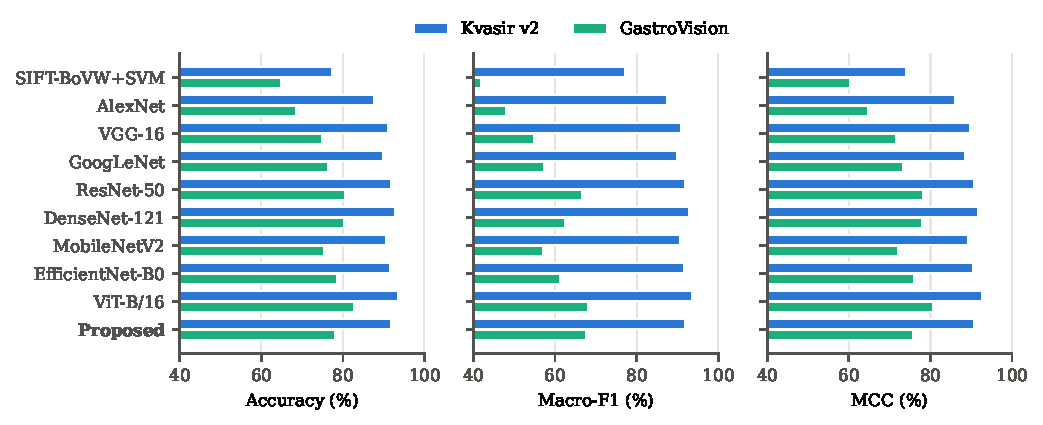
\includegraphics[width=\textwidth]{fig_baseline_comparison.pdf}
\caption{Baseline comparison on the two classification databases (test sets). The proposed system is the
bottom row of each panel.}
\label{fig:bars}
\end{figure*}

\begin{figure*}[t]
\centering
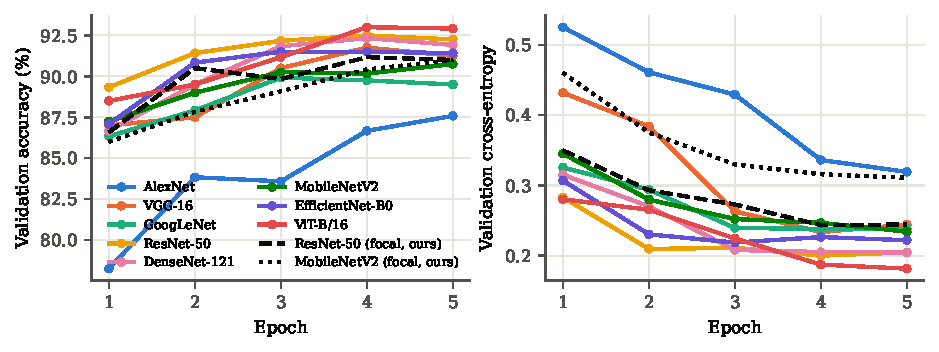
\includegraphics[width=\textwidth]{fig_training_curves.pdf}
\caption{Validation accuracy and cross-entropy per epoch on Kvasir v2 for all deep baselines and for the two
focal-loss stages of the proposed system (black).}
\label{fig:curves}
\end{figure*}

The confusion matrices (Fig.~\ref{fig:confusion}) show that the dominant error on Kvasir is the confusion between
\emph{oesophagitis} and the \emph{normal Z-line}, and between \emph{dyed-lifted polyps} and \emph{dyed resection
margins}. Both pairs are visually near-identical and are known to be ambiguous even for annotators, which is also
visible in the per-class F1 scores (Fig.~\ref{fig:perclass}). The ROC curves (Fig.~\ref{fig:roc}) show
micro-averaged AUCs above 0.99 for all deep models on Kvasir.

\begin{figure*}[t]
\centering
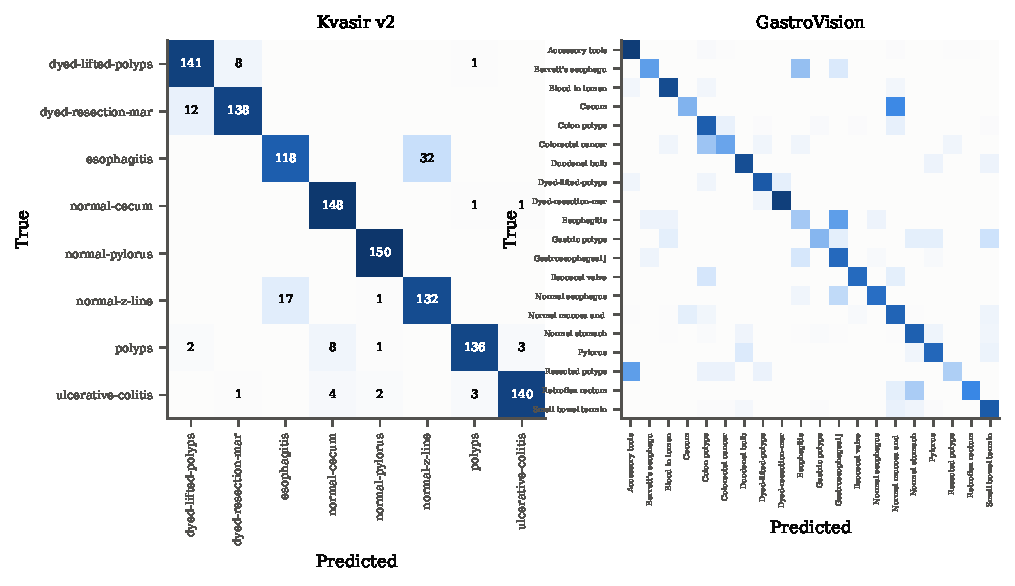
\includegraphics[width=\textwidth]{fig_confusion.pdf}
\caption{Confusion matrices of the proposed cascade on the clean test sets (rows: true class).}
\label{fig:confusion}
\end{figure*}

\begin{figure*}[t]
\centering
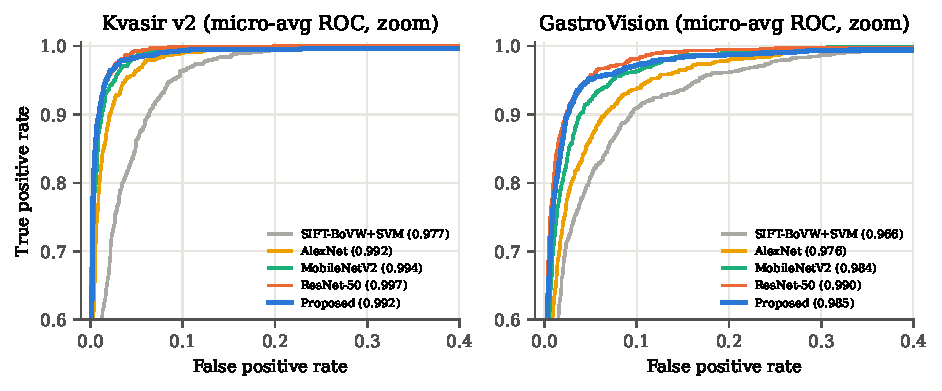
\includegraphics[width=\textwidth]{fig_roc.pdf}
\caption{Micro-averaged ROC curves (zoomed into the upper-left corner) with AUC in brackets.}
\label{fig:roc}
\end{figure*}

\begin{figure}[t]
\centering
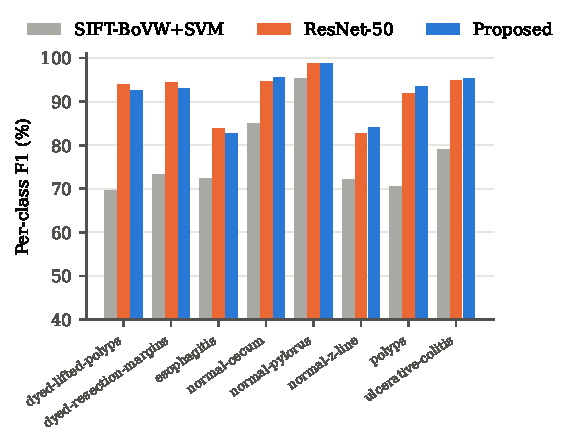
\includegraphics[width=\linewidth]{fig_perclass_f1.pdf}
\caption{Per-class F1 on Kvasir v2.}
\label{fig:perclass}
\end{figure}

\subsection{Generalisation to a Second Classification Database}
Table~\ref{tab:multidb} repeats the comparison on GastroVision, which covers more classes (including gastric
findings) and is strongly imbalanced. Here plain accuracy is dominated by the large classes, so balanced accuracy and
MCC are the more informative evaluators. The proposed cascade obtains \Rgastrovisionacc\% accuracy and
\Rgastrovisionbalacc\% balanced accuracy (best baseline: \Rgastrovisionbestbase, \Rgastrovisionbestbaseacc\% /
\Rgastrovisionbestbasebacc\%). The classical baseline collapses on this database, especially in balanced accuracy,
because its fixed descriptors cannot separate the many fine-grained classes. Although its plain accuracy is lower than that of the
strongest single-frame networks, the proposed cascade has the highest balanced accuracy of all methods, i.e.\ the best
recall on the rare classes, which is the intended effect of the focal loss and the abnormality-oriented gate.

\maybeinput{tables/multi_db}

\subsection{Robustness to Endoscopic Artifacts}
\label{sec:robust}
Table~\ref{tab:robust} and Fig.~\ref{fig:robust} report Kvasir accuracy when the current frame is hit by a
transient artifact. Every single-frame model degrades sharply, because it has nothing to classify except the
corrupted frame: averaged over the four artifact types, the most robust baseline (\Rrobbestbase) keeps only
\Rrobbestbaseacc\%, and ResNet-50 keeps \Rresnettransient\%. The proposed system keeps \Rrobtransient\%, essentially
its clean accuracy, and \Rrobstream\% on a random artifact stream where 30\% of all frames are corrupted. This is the
behaviour the temporal stage was designed for: a lesion that is visible in the preceding frames is not lost because of
one blurred or flashed frame, and an artifact cannot create a lesion that the preceding frames do not show.

\maybeinput{tables/robustness}

\begin{figure*}[t]
\centering
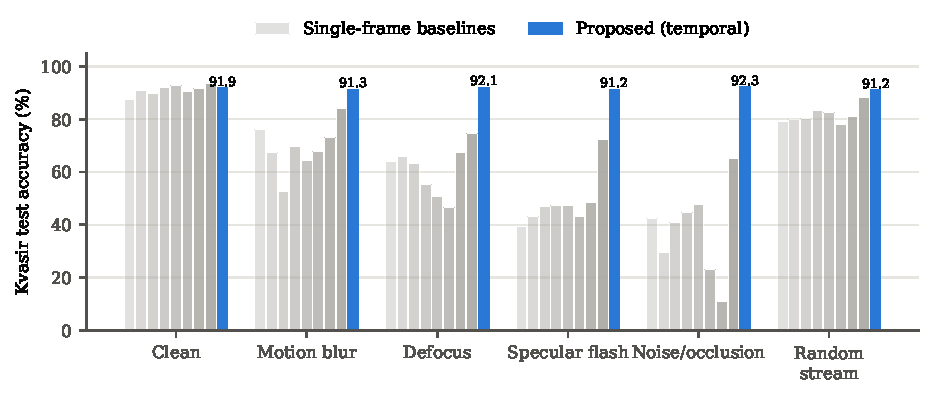
\includegraphics[width=\textwidth]{fig_robustness.pdf}
\caption{Kvasir test accuracy under transient artifacts on the current frame and on a random artifact stream.
Grey bars: the eight single-frame deep baselines (left to right as in Table~\ref{tab:main}); blue: proposed.}
\label{fig:robust}
\end{figure*}

Fig.~\ref{fig:attention} shows why: the learned temporal attention $a_t$ assigns corrupted frames an average weight
an order of magnitude lower than clean frames at every position of the window, i.e.\ the Bi-LSTM has learned
\emph{which} frames to trust without any frame-quality supervision.

\begin{figure}[t]
\centering
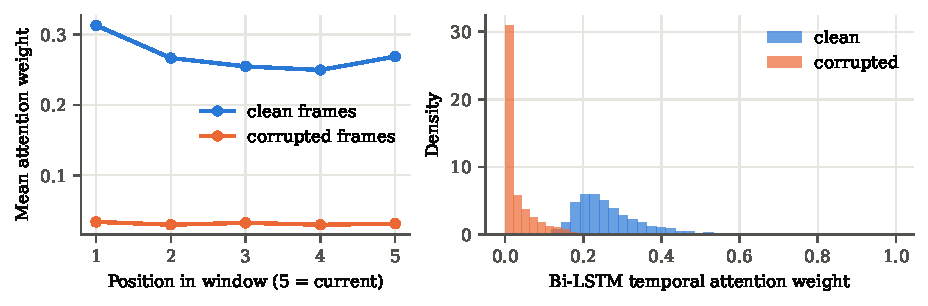
\includegraphics[width=\linewidth]{fig_attention.pdf}
\caption{Bi-LSTM temporal attention on the artifact stream: mean weight per window position (left) and the
distribution of weights (right) for clean versus corrupted frames.}
\label{fig:attention}
\end{figure}

\subsection{Ablation Study}
Table~\ref{tab:ablation} isolates each component. (i) Replacing cross-entropy by focal loss changes clean Kvasir
accuracy only marginally on this balanced database. (ii) Any form of temporal aggregation removes most of the artifact
sensitivity of the single-frame model. Simple mean pooling of the per-frame probabilities is a strong baseline on our
synthetic clips, because neighbouring frames are near-duplicates; the Bi-LSTM performs comparably while additionally
providing interpretable attention weights and the capacity to model genuine appearance changes in real video.
(iii) Routing on the \emph{current} frame only makes the gate itself the weak point: a flash or a dark occlusion can
push a lesion frame below $\tau$ and cause a bypass. Averaging the gate probabilities over the five-frame buffer
(gate scores are computed once per frame anyway) removes this failure mode at no extra cost, and the full cascade
matches the un-gated temporal model while skipping Stages 2--3 for part of the stream.

\maybeinput{tables/ablation}

\subsection{Computational Efficiency and the Stage-1 Gate}
The gate threshold is selected on validation data as the largest $\tau$ that keeps the abnormal-frame recall at
$\ge$99.5\% (Fig.~\ref{fig:tau}); this gives $\tau=\Rtau$ on Kvasir, a test-set gate recall of \Rgaterec\% for
abnormal frames and a bypass rate of \Rbypass\% of all frames (Table~\ref{tab:gate}). Measured on the idle M5 GPU at
batch size 1, the gate costs \Rgatems~ms and Stages 2--3 cost \Rstagems~ms per frame, so the expected cost of the
cascade at Kvasir's class mix is \Rcasms~ms (\Rcasfps~FPS) and \Rcasgmacs~GMACs, against \Rressinglems~ms and
\Rgmacsresnet~GMACs for ResNet-50 on every frame: at this prevalence the cascade roughly breaks even, while adding the
temporal verification for free. On the CPU, PyTorch's depthwise-convolution kernels for this ARM processor are
inefficient (MobileNetV2 is slower than ResNet-50 despite needing 13$\times$ fewer MACs), so the gate brings no CPU
wall-clock gain without an optimised mobile runtime; CPU figures are nevertheless reported in Table~\ref{tab:main}.

\begin{figure}[t]
\centering
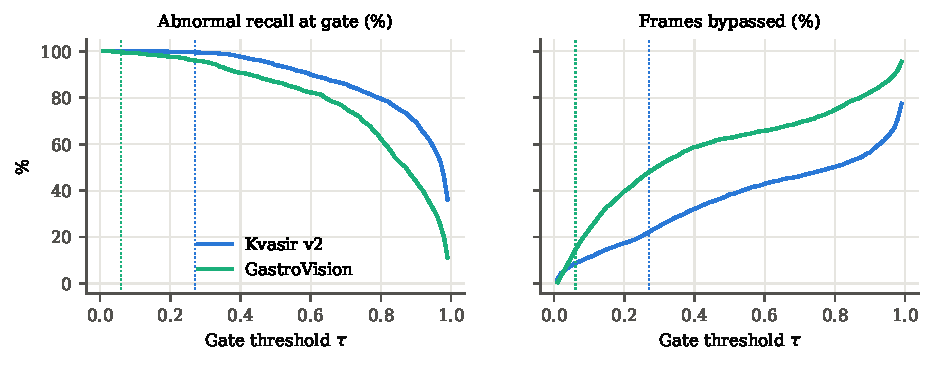
\includegraphics[width=\linewidth]{fig_tau_sweep.pdf}
\caption{Gate threshold sweep on the validation sets: recall of abnormal frames and fraction of bypassed frames.
Dotted lines mark the selected $\tau$.}
\label{fig:tau}
\end{figure}

\maybeinput{tables/gate}

The benefit of the cascade grows with the fraction of normal frames in the stream (Fig.~\ref{fig:prevalence}).
Kvasir is a curated, class-balanced benchmark in which only 3 of 8 classes are normal, whereas most frames of a full
screening examination show normal mucosa. With 80\% normal frames the expected cost falls to \Rcasgmacseighty~GMACs
(\Rcasgpueighty~FPS on the GPU), and with 90\% normal frames to \Rcasgmacsninety~GMACs (\Rcasgpuninety~FPS), compared
with \Rgmacsresnet~GMACs / \Rfpsresnet~FPS for ResNet-50 and \Rgmacsvitb~GMACs / \Rfpsvitb~FPS for ViT-B/16 applied
to every frame. Fig.~\ref{fig:tradeoff} places all models in the accuracy--throughput plane.

\begin{figure*}[t]
\centering
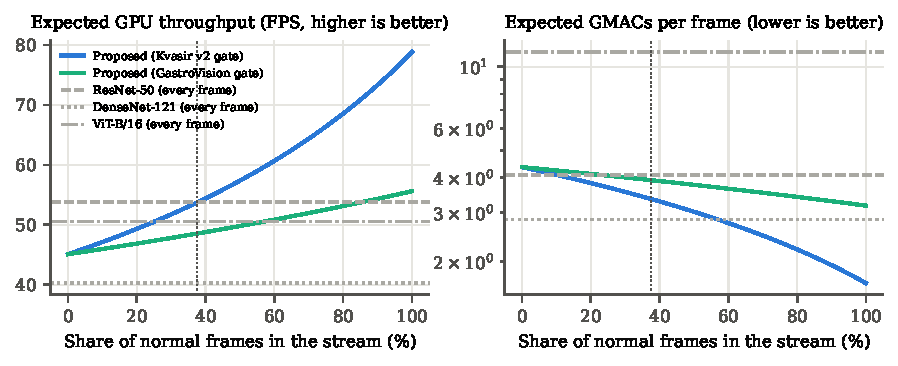
\includegraphics[width=\textwidth]{fig_prevalence.pdf}
\caption{Expected cascade cost as a function of the share of normal frames, computed from the measured component
latencies and the gate's measured recall/specificity: GPU throughput (left) and GMACs per frame (right, log scale).
Grey lines are single-frame baselines run on every frame; the dotted line marks Kvasir's test prevalence.}
\label{fig:prevalence}
\end{figure*}

\begin{figure}[t]
\centering
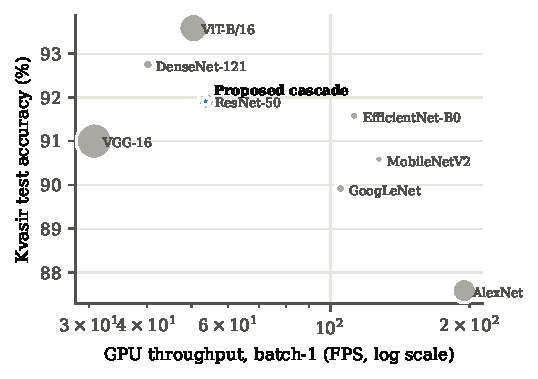
\includegraphics[width=\linewidth]{fig_accuracy_vs_fps.pdf}
\caption{Accuracy versus batch-1 GPU throughput on Kvasir v2 (marker area $\propto$ parameters).}
\label{fig:tradeoff}
\end{figure}

\subsection{Cross-Database Generalisation}
Table~\ref{tab:cross} applies the Kvasir-trained models, without any re-training, to the two pixel-annotated polyp
databases. Kvasir-SEG images are drawn from the same source as Kvasir, so its numbers mainly measure in-domain
consistency; \Rkvasirsegn\ of \Rkvasirsegntotal\ images remain after removing near-duplicates of training images.
CVC-ClinicDB comes from a different hospital and endoscope and is therefore a true domain-shift test. On CVC-ClinicDB
the proposed cascade flags \Rcvcprop\% of the polyp frames as abnormal (\Rcvcproppolyp\% as \emph{polyp}). The
gap between the polyp-class and abnormal-class sensitivities shows that many shifted-domain polyps are still routed to
the lesion branch even when the fine-grained label is wrong, which is the clinically relevant behaviour for a
detection aid. ViT-B/16 and EfficientNet-B0 transfer best to the new domain, which suggests that the Stage-2
backbone, rather than the temporal design, limits cross-domain robustness; on the in-domain Kvasir-SEG images the
proposed cascade has the highest polyp sensitivity (\Rkvasirsegproppolyp\%).

\maybeinput{tables/crossdata}

\subsection{Explainability}
Grad-CAM maps of the Stage-2 network (Fig.~\ref{fig:gradcam}) are compared quantitatively with the expert polyp
masks in Table~\ref{tab:gradcam}. The pointing-game hit rate of the proposed Stage-2 network is \Rgckvasirsegpg\% on
Kvasir-SEG and \Rgccvcpg\% on CVC-ClinicDB, against a random-pointing baseline equal to the mean mask area
(\Rgckvasirsegarea\% and \Rgccvcarea\%). This indicates that the network attends to the lesion itself rather than to
dataset artifacts such as the green position-indicator box or text overlays. Interestingly, the cross-entropy ResNet-50
localises slightly better than the focal-loss version on both databases: focal loss down-weights easy, confidently
classified polyps, which yields lower-confidence and somewhat more diffuse maps; this trade-off between rare-class
sensitivity and map sharpness is worth further study. Finally, the t-SNE embedding
\cite{vandermaaten2008tsne} of the Stage-2 features (Fig.~\ref{fig:tsne}) shows compact class clusters, with the
expected overlap between oesophagitis and Z-line and between the two dyed classes.

\maybeinput{tables/gradcam}

\begin{figure*}[t]
\centering
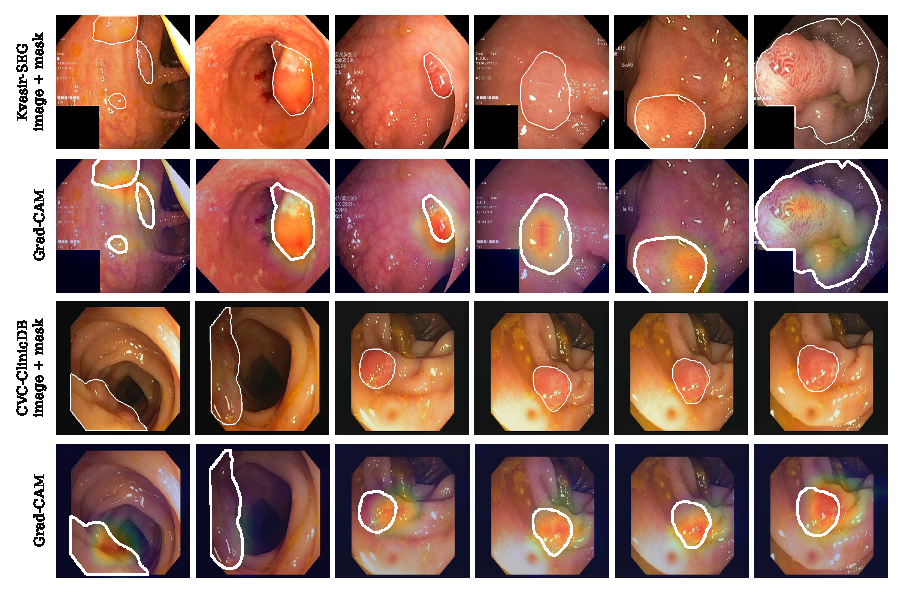
\includegraphics[width=\textwidth]{fig_gradcam.pdf}
\caption{Grad-CAM of the proposed Stage-2 network for the \emph{polyp} class on unseen Kvasir-SEG and CVC-ClinicDB
frames; the expert polyp mask is outlined in white. The map is scaled by the model's confidence.}
\label{fig:gradcam}
\end{figure*}

\begin{figure}[t]
\centering
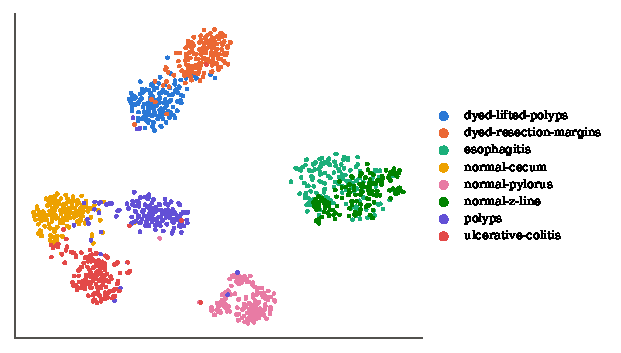
\includegraphics[width=\linewidth]{fig_tsne.pdf}
\caption{t-SNE of the 2048-d Stage-2 features of the Kvasir test images.}
\label{fig:tsne}
\end{figure}

\subsection{Limitations}
The temporal clips are synthesised from still images, so the study measures robustness to \emph{simulated}
artifacts; evaluating on real annotated video (e.g.\ the HyperKvasir video collection \cite{borgli2020hyperkvasir}) is the most important next step.
All networks were fine-tuned for a short, fixed budget on a single train/validation/test split; repeated runs with
different seeds would provide confidence intervals. Rare classes with fewer than 30 images, including gastric
ulcers in GastroVision, had to be excluded, which also limits the strength of the claims for rare gastric
pathologies.
